\documentclass{article}
\usepackage[backend=bibtex]{biblatex}
\usepackage{hyperref}
\usepackage{graphicx}
\addbibresource{bibliography.bib}
\graphicspath{ {images/} }

\begin{document}


\title{ChIP-seq data analysis of Sin3A in Drosophila melanogaster}
\author{Fien Strijthaegen
\\Université Libre de Bruxelles
\\MA1 Bioinformatics and modelling}
\date{August 24th, 2023}
\maketitle

\section{Introduction}
%Tutorials: 
%https://github.com/hbctraining/Intro-to-ChIPseq-flipped
%https://bioinformatics-core-shared-training.github.io/cruk-summer-school-2021/ChIPSeq/practicals/ChIP_Practical3_DownstreamAnalysis_2021.html

Chromatin immunoprecipitation followed by sequencing (ChIP-seq) is a method in epigenomic research for the analysis of binding sites of DNA-associated proteins. DNA and associated proteins on chromatin are crosslinked, then the DNA-protein complexes are sheared into small fragments. The fragments associated with the protein of interest are selectively immunoprecipitated using a protein-specific antibody and then purified and sequenced. Computational analysis of these sequenced reads can reveal epigenomic information\cite{nakato2021methods}. The ENCODE consortium\cite{de2012encode} hosts several databases of biological assays, including ChIP-seq of several species. 

In this project, an analysis was performed on a data set of the Kc167 cell line of Drosophila melanogaster from the ENCODE ChIP-seq database, targeting the Sin3A gene. This gene encodes the paired amphipathic helix protein of the same Sin3A, a transcriptional regulatory protein. The analysis was guided by practice sessions from this course as well as a HCB \cite{meeta2023hbctraining} and \href{https://bioinformatics-core-shared-training.github.io/cruk-summer-school-2021/ChIPSeq/practicals/ChIP_Practical3_DownstreamAnalysis_2021.html}{CRUK} course.

TODO: summary

\section{Data sets}
This analysis concerns data from Encode experiment \href{https://www.encodeproject.org/experiments/ENCSR264MBG/}{ENCSR264MBG}, the reads of which were sequences on the Illumina HiSeq 2000 platform. The analysis was performed on isogenic replicate 1 and 2. The reads are single-ended, with a length of 44 nucleotides. The genome assembly of Drosophila melanogaster was acquired from the UCSC genome browser\cite{karolchik2003ucsc}. The soft-masked assembly from the file \href{https://hgdownload.soe.ucsc.edu/goldenPath/dm6/bigZips/}{dm6.fa.gz} was used in the analysis. The BED file \href{https://github.com/Boyle-Lab/Blacklist}{dm6-blacklist.v2.bed.gz} with blacklisted regions was acquired from the Boyle Lab\cite{amemiya2019encode}. The database used for MEME-Chip analysis was OnTheFly_2014_Drosophila.meme\cite{shazman2014onthefly}, which contains 608 motifs, between 4 and 23 in width, with an average width of 9.3. 

\section{Code availability}
TODO

\section{Analysis}

\subsection{Read mapping}

% OPTIONAL: quality plots for reads (lesson 3 workshop)
Code for this section is in the R script read\_mapping.R. The raw FASTQ files contain reads of length 44nt, 23 million for isogenic replicate 1, and 18 million for isogenic replicate 2. The ends of these reads were trimmed based on quality, ends with a quality score lower than 20 were trimmed. Reads with a length lower than 40nt were filtered out. This filtering was performed using the ShortRead package\cite{morgan2009shortread}.

Reads were mapped to the assembled genome using the Rsubread package\cite{liao2019r} with default parameters. Then filtering was performed using Sambamba\cite{tarasov2015sambamba}. Unmapped reads, duplicates and multimapped reads were filtered out, leaving only uniquely mapping reads. While including multi-mapped reads would increase the number of usable reads and might increase the sensitivity of peak detection, they were omitted here, following convention, since the number of false positives might also increase\cite{chung2011discovering}.

%OPTIONAL: mapping stats

%Mapping statistics were calculated using the program Samtools\cite{li2009sequence}. Figure \ref{fig:coverage} contains a histogram of the read coverage. The average coverage is TODO. 21.166.296 reads were mapped to the genome for isogenic replicate 1, and TODO for isogenic replicate 2. 


\subsection{Peak calling}


%on cli:
% $ macs2 callpeak -t ../filtered_ENCFF515LPH.bam -n ENCFF515LPH
% $ bedtools intersect -v -a ENCFF515LPH_peaks.narrowPeak -b ../dm6-blacklist.v2.bed.gz > noblacklist_ENCFF515LPH.bed
% $ bedtools intersect -wo -f 0.3 -r -a noblacklist_ENCFF515LPH.bed -b noblacklist_ENCFF708WHR.bed > overlapping.bed
% $ bamCoverage -b filtered_ENCFF708WHR.bw -o filtered_ENCFF708WHR.bw
% $ computeMatrix reference-point --referencePoint center -b 2000 -a 2000 -R macs2/overlapping.bed -S filtered_ENCFF515LPH.bw filtered_ENCFF708WHR.bw -o matrix.gz --missingDataAsZero
% $ plotHeatmap -m matrix.gz -out heatmap4.png

Peak calling was performed with MACS2\cite{gaspar2018improved} using default parameters. Bedtools\cite{quinlan2010bedtools} was used to filter out blacklisted regions from the results. Removing these anomalous, unstructured or high in signal independent of cell line or experiment regions improves accuracy\cite{amemiya2019encode}. Concordance between replicates was then assessed by finding overlapping regions. Regions that overlap at least 30\% between the results of isogenic replicates 1 and 2 were kept for further analysis. Deeptools\cite{ramirez2014deeptools} was used to visualize the signal. Figure \ref{fig:heatmap} shows that there is a signal for both isogenic replicates. TODO: more explanation.

\begin{figure}[h]
\caption{Profile plot and heatmap of both isogenic replicates.}
\centering
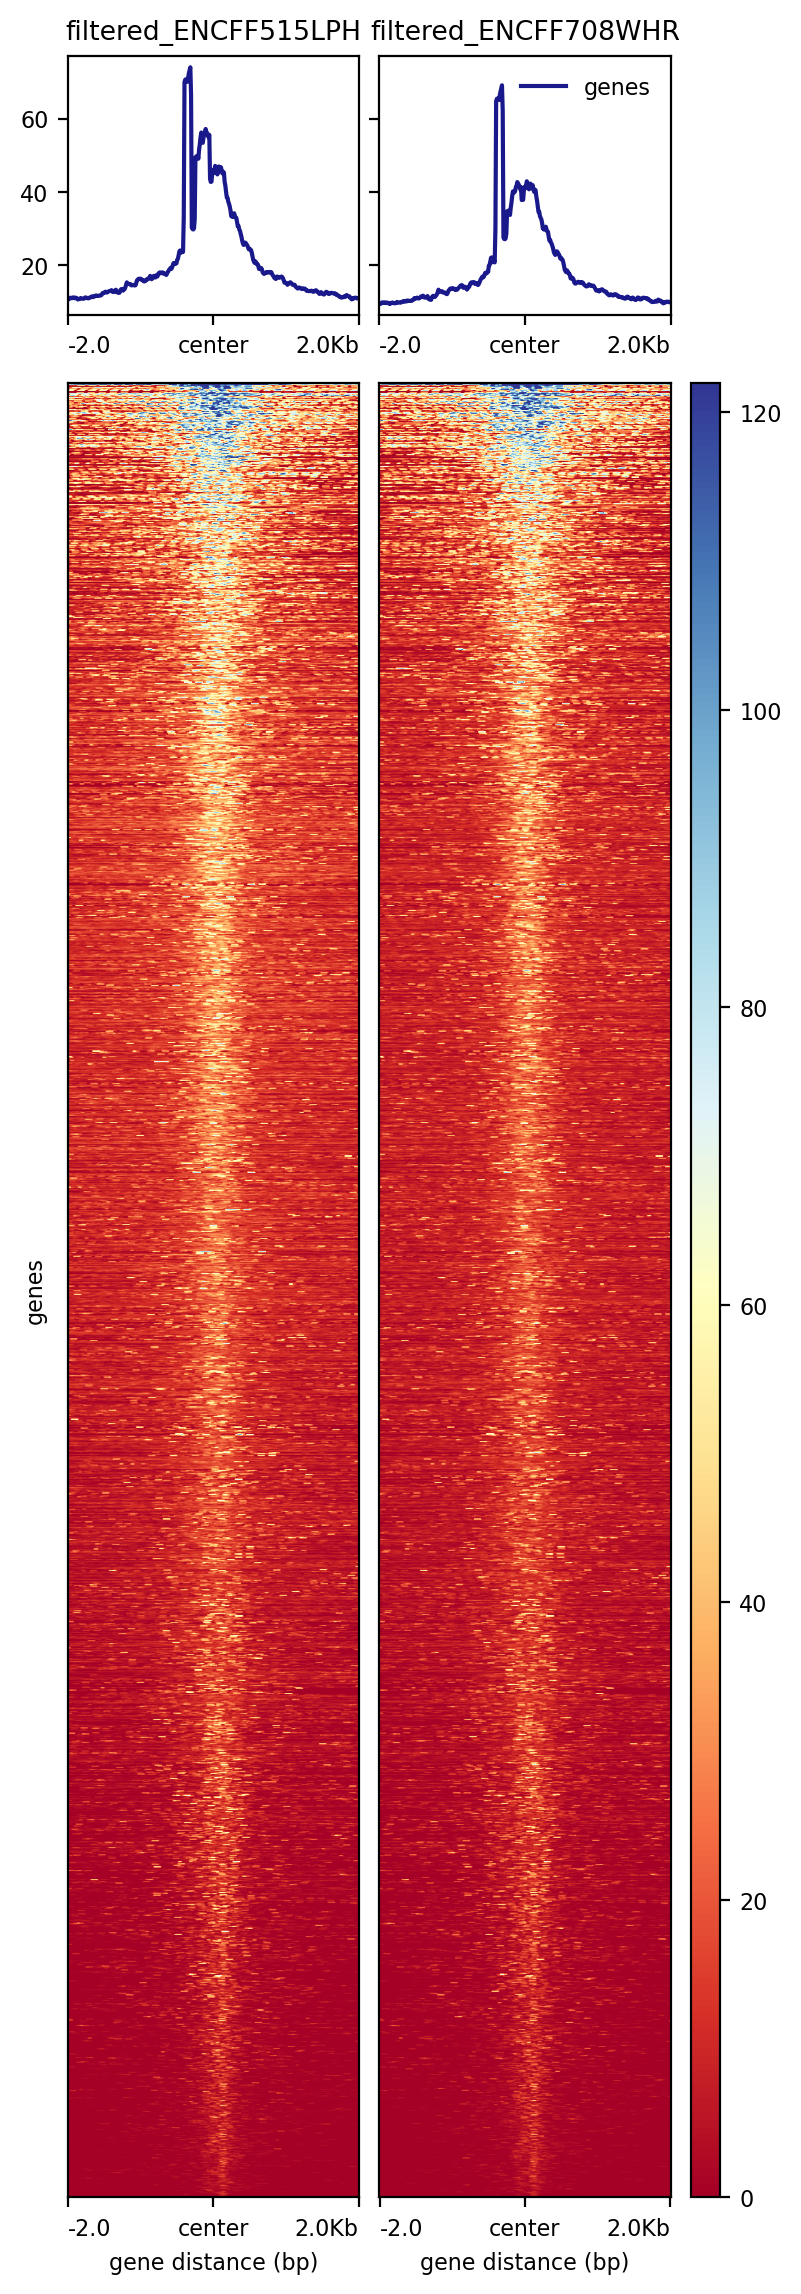
\includegraphics[height=\textheight]{heatmap.png}
\label{fig:heatmap}
\end{figure}

\subsection{Annotation and functional enrichment analysis}
ChIPseeker\cite{yu2015chipseeker} was used to annotate genomic features. Figures \ref{fig:feat_dist} and \ref{feat_TSS} visualize the distances from the peak to the transcription start site of the nearest genes. TODO: describe.

\begin{figure}[h]
\caption{Feature distribution}
\centering
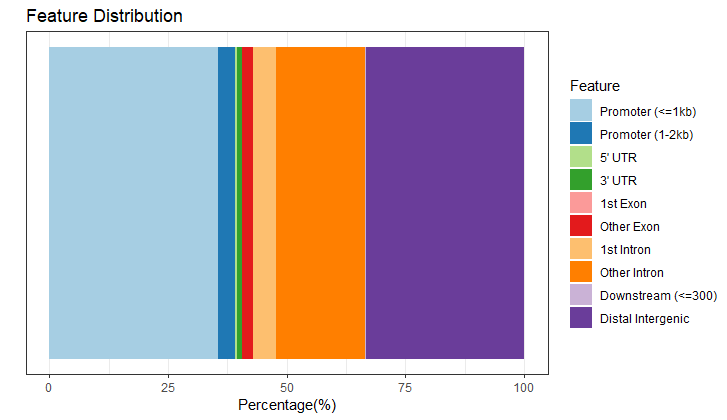
\includegraphics{feature_distribution.png}
\label{fig:feat_dist}
\end{figure}

\begin{figure}[h]
\caption{Feature distribution TSS}
\centering
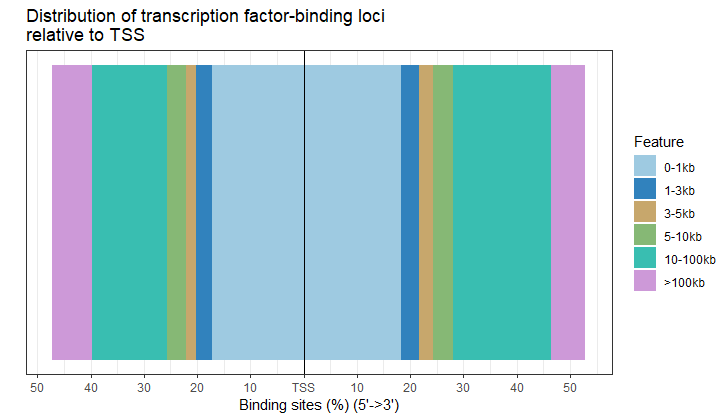
\includegraphics{feature_distribution_TSS.png}
\label{fig:feat_TSS}
\end{figure}

ReactomePA\cite{yu2016reactomepa} was used for functional enrichment analysis. Figure \ref{fig:pathways} displays the gene sets found. TODO: describe gene sets.

\begin{figure}[h]
\caption{Pathways}
\centering
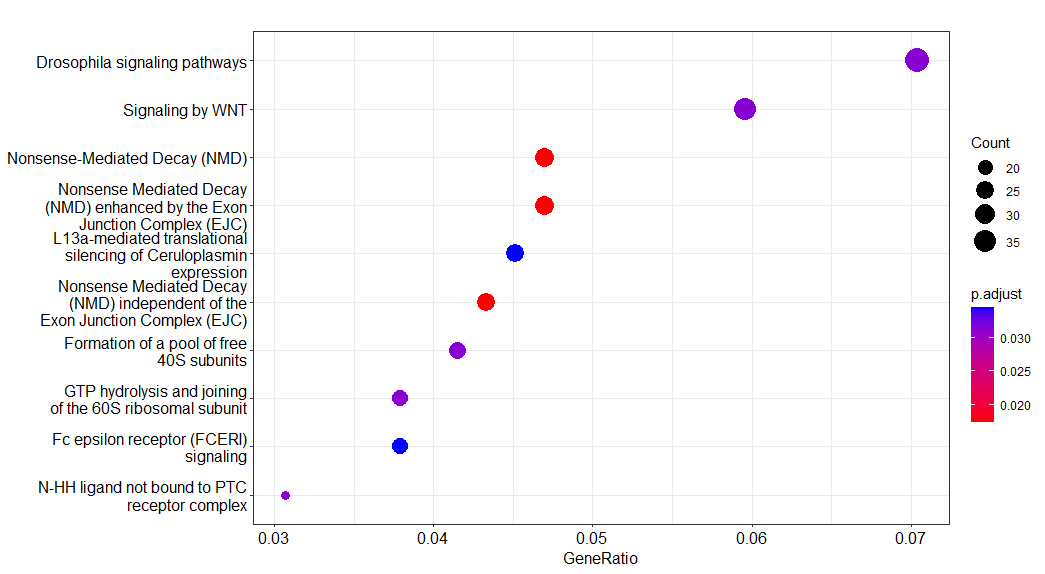
\includegraphics{pathways.png}
\label{fig:pathways}
\end{figure}

\subsection{Motif discovery and annotation}
% >docker run -v D:\GitHub\ChIP-seq-project:/home/meme -d memesuite/memesuite:latest

The CLI version of MEME-Chip\cite{machanick2011meme} was used to perform motif discovery. 


% $ bedtools getfasta -fi ../dm6.fa -bed overlapping.bed -fo overlapping.fa
% $ meme-chip -oc meme_output -db motif_databases/FLY/OnTheFly_2014_Drosophila.meme macs2/overlapping.fa

\section{Conclusion}
Future work:
inclusion multi-mapped reads\cite{chung2011discovering}

\printbibliography

\appendix

\end{document}
